\documentclass[openany,12pt]{report}

\setlength{\textwidth}{6.25in} % original 6.25

\setlength{\textheight}{8.9in}

\renewcommand{\baselinestretch}{1.3}

%\headheight 12.0pt

\oddsidemargin 20pt    %  Left margin on odd-numbered pages.

\evensidemargin 20pt   %  Note that \oddsidemargin = \evensidemargin

\topmargin 0pt

%\headsep 10pt

\footskip 10.0pt

\usepackage {graphics}

%\usepackage {algorithm}

%\usepackage {algorithmic}
\usepackage{hyperref}
\usepackage{color}
\usepackage{lastpage} % for the number of the last page in the document
\usepackage{fancyheadings}
\pagestyle{fancy}
\usepackage {epsfig}
\usepackage {graphicx}
\usepackage{float}
\usepackage{array} % for making text bold in table
\usepackage{longtable}
%\usepackage[dvips, bookmarks, colorlinks=false]{hyperref}
%\usepackage{hyperref} %for creating links in the pdf version and other additional pdf attributes, no effect on the printed document
\usepackage{lipsum}
%*****************************Title Page**************************************************************

\begin{document} % Begin document "environment".


 
\lhead{}
\chead{}
\rhead{Cryptocurrency Research And Analytical Tool}
\lfoot{ MET's Institute of Engineering}
\setlength{\headrulewidth}{0.4pt}
\setlength{\footrulewidth}{0.4pt}
\fontsize{12}{15}
\begin{titlepage}
\begin{center}
%\vspace{0.2in}
{\bf A Project Report on} \\
\vspace{0.3in}
{\Large \bf ``Cryptocurrency Research And Analytical Tool''}\\
\vspace{0.3in}
SUBMITTED TO THE SAVITRIBAI PHULE UNIVERSITY, PUNE\\
IN THE PARTIAL FULFILLMENT OF THE REQUIREMENTS \\
FOR THE AWARD OF THE DEGREE \\
\vspace{0.2in}
OF\\  
\vspace{0.2in}
BACHELOR OF ENGINEERING (COMPUTER ENGINEERING)\\
(Academic Year: 2021-22)\\
\vspace{0.2in}

{\it SUBMITTED BY}\\

\vspace{0.2in}

{\bf Mr. Vedant D. Mulherkar}\hspace{0.32in} {\bf (Exam Seat No: B150474273)} \\

{\bf Mr. Ganesh C. Vispute     }\hspace{0.5in}{\bf (Exam Seat No: B150474318)}\\  \\
{\bf Mr. Avinash P. Mankar    }\hspace{0.43in}{\bf (Exam Seat No: B150474201)}\\  \\

\vspace{0.4in}

{\it Under the guidance of}\\

\vspace{0.1in}

{\bf Mr. Sandip A. Kahate}\\
\vspace{0.4in}


{\small DEPARTMENT OF COMPUTER ENGINEERING}\\
\begin{figure*}[h]
\centerline{\psfig{figure=./metbkc.eps,width=4.1in,height=0.5in}}
\label{atcres}
\end{figure*}
{\large MET's Institute of Engineering,}\\
{\small Adgaon, Nashik-422003}\\
SAVITRIBAI PHULE PUNE UNIVERSITY,PUNE \\
\vspace{0.2in}

\vspace{0.1in}
{\bf May 2022}\\
\vspace{0.4in}

\end{center}
\end{titlepage}

%*****************************Certificate*************************************************************
\fontsize{14}{16}
\thispagestyle{empty}
\begin{center}
\begin{figure*}[h]
\centerline{\psfig{figure=./metbkc.eps,width=7.2in,height=1.2in}}
\label{atcres}
\end{figure*}
\vspace{0.1in}
{\it \Huge  \textbf{Certificate}}\\
\vspace{0.2in}
{\it This is to Certify that the project report entitles}\\
\vspace{0.2in}
{\Large \bf ``Cryptocurrency Research And Analytical Tool''}\\
\vspace{0.2in}
\textbf{Submitted by}}
\vspace{0.2in}

{\bf Mr. Vedant D. Mulherkar}\hspace{0.32in} {\bf (B150474273)} \\

{\bf Mr. Ganesh C. Vispute     }\hspace{0.5in}{\bf (B150474318)}\\  \\
{\bf Mr. Avinash P. Mankar    }\hspace{0.5in}{\bf (B150474201)}\\  \\
\end{center}
\vspace{0.3in}
{\it are bonafide students of this institute and the work has been carried out by them under
the guidance of Mr. Sandip A. Kahate and it is approved for the partial fulfillment of the
requirement of Savitribai Phule Pune University for the award of the degree of Bachelor
of Engineering (Computer Engineering).}\\
\vspace{0.2in}
\vspace{0.7in}
\noindent

\hspace{0.1in} Project Guide  \hspace{1.5in}H.O.D \hspace{0.9in} Principal  \\
\hspace{4.6in} (Mr. Sandip A. Kahate) \hspace{0.6in}(Dr. M. U. Kharat)\hspace{0.4in}(Dr. V. P. Wani)\\

\vspace{0.1in}

Place: Nashik

Date: \hspace{0.2in}/\hspace{0.3in}/   \\
\\
\newpage \pagenumbering{roman}
%\vskip
\chapter*{Acknowledgements}

We have taken efforts in this project. However, it would not have been possible without the kind support and help of many individual and organizations. We would like to extend our sincere thanks to all of them. It gives us proud privilege to complete the project on \textbf{ ``Cryptocurrency Research And Analytical Tool''}. We are highly indebted to our internal guide \textbf{Mr. Sandip A. Kahate} for his guidance and constant supervision as well as for providing necessary information regarding the project and also for his support in completing the project.\\
\hspace*{0.5in}We are also extremely grateful to our respected H.O.D. (Computer Department) \textbf{Dr. M. U. Kharat}  and  \textbf{Dr. Priti N. Metange} (Project Coordinator) for providing all facilities and every help for smooth progress of project work.\\
\\
\\
\\
\\
\\
\\
\hspace*{4.0in} Mr. Vedant Mulherkar\\
\hspace*{4.0in} Mr. Ganesh Vispute \\
\hspace*{4.0in} Mr. Avinash Mankar
\\
\\
\\
\\
\\
\\
\\


%*****************************Abstract*************************************************************
\chapter*{Abstract\markboth{Abstract}{Abstract}}

Growing demand in internet usage has bring up to the revolution in digital economy. From the past decade digital economy is playing major role round the world. 
The physical assets are converted to digital assets, in which crypto currency is playing prime role.
Now day world’s billionaires and millionaires want to invest into cryptocurrency instead of stocks like Elon musk . 
A cryptocurrency, crypto-currency, or crypto is a binary data designed to work as a medium of exchange wherein individual coin ownership records are stored in a ledger existing in a form of a computerized database using strong cryptography to secure transaction records, to control the creation of additional coins and to verify the transfer of coin ownership.
Crypto currency price prediction and forecast has been one of the tedious tasks for long period. Existing works are attempted to go for accurate prediction and forecast through machine learning models.
The forecast can be useful work for the investors to know about the nature of price in future and gives them directions for their investments.
In this proposed work, crypto price prediction is proposed through the machine learning models such as Artificial Neural Network and Long short-term memory (LSTM) models.
With Prediction user get the benefits of crypto comparison  and crypto conversion, With the use of the data analysis we try to analyses past value of more than two cryptocurrencies and give their comparison.
\\
\\
With the use of this  program investor will able perform crypto-to-crypto conversion.The aim of the work is to give accurate predictions and forecast with comparison and conversion to bring the daily trend for crypto currency in market.
Experimental studies shows that the proposed technologies of machine learning give better accuracy on predictions.
\\
\\
Keywords: Crypto-currency, Machine learning, 
Long short term memory (LSTM),\\Analysis,Comparison, Conversion.

\newpage
\tableofcontents
\listoffigures
\listoftables
\newpage	
\pagenumbering{arabic}





%*****************************Chapter1 *****************************

\chapter{Introduction}
This chapter describes the terms related to Prediction of cryptocurrency and to forecast cryptocurrency prices using all the trading features
like price, volume, open, high, low values present in the dataset. \\
\section{Overview}
Cryptocurrency, sometimes called crypto-currency or crypto. It is a form of currency that exists digitally or virtually and uses cryptography to secure transactions. Cryptocurrencies don't have a central issuing or regulating authority instead using a decentralized system to record transactions and issue new units.
Where Cryptography is the study of secure communications techniques that allow only the sender and intended recipient of a mess or code to view its contents.Here, data is encrypted using a secret key, and then both the encoded message and secret key are sent to the recipient for decryption.
A pseudonymous computer scientist called Satoshi Nakamoto proposed bitcoin for the first time in 2008. The main purpose of this digital currency has been to use it as means of exchange, independent of any central authority. By encrypting every single bitcoin with advanced mathematical principles, secure electronic transactions are ensured by cryptocurrency miners. Although it is a legit usage, any digital cryptocurrency might usually be called as ‘Bitcoin’ among the traders since Bitcoin is the first cryptocurrency with the highest amount of market capital 962 billion dollars in the market in December 2021. However, in the market, there are as many as 8000 different cryptocurrencies in 2021 with different names (‘Ethereum’, ‘Ripple’, ‘Litecoin’…) and constantly new ones

are created.
Especially, massive fluctuations in the prices of all cryptocurrencies have no doubt kept attention. In 2008, when bitcoin was first introduced, its price was below 1 dollar. Growing slowly in a usual trend, its price hit 1000 dollar in February 2017 for the first time. Until August 2017, its price quadrupled in a short interval keeping global attention. Cryptocurrencies price is renowned for being highly volatile, but despite that, it has become the top performing asset of any class (including stocks, commodities and bonds) over the past decade – climbing a staggering 9,000,000 percent between 2010 and 2020.
When the cryptocurrency was launched at the beginning of 2009, as Satoshi Nakamoto mined the bitcoin genesis block (the first-ever block on the Bitcoin blockchain), 50 BTC entered circulation at a price of 0.00 dollors (coindesk.com, 2021).
Even after the cryptocurrency has undergone several rallies and crashes since it become available then also its popularity not fall.Bitcoin's last peak was near 14,000 dollors in June of 2019.
At this point, Bitcoin with other currencies experienced a hard resistance it failed to push through this stage due to which other cryptocurrencies take advantage and started to group up.This events shows us the volatile nature of cryptocurries and show us the difficulty to predict the growth of fall of a crypto.\\ 
Although machine learning has been successful in predicting stock market prices through a host of different time series models, its application in predicting cryptocurrency prices has been quite restrictive. The reason behind this is obvious as prices of cryptocurrencies depend on a lot of factors like technological progress, internal competition, pressure on the markets to deliver, economic problems, security issues, political factor etc. Their high volatility leads to the great potential of high profit if intelligent inventing strategies are taken. Unfortunately, due to their lack of indexes, cryptocurrencies are relatively unpredictable compared to traditional financial predictions like stock market prediction.
\\
The model validate and tested whether the predictions are good even when the market direction changes .\\
Figure 1.1 . shows the flow of the software and how it loaded with various stages from dataset generation to data prediction from data  processing to data analysis show the magic of machine learning in this application which makes the result easy to predict.

\\
\\
\begin{figure}[H]
\centering
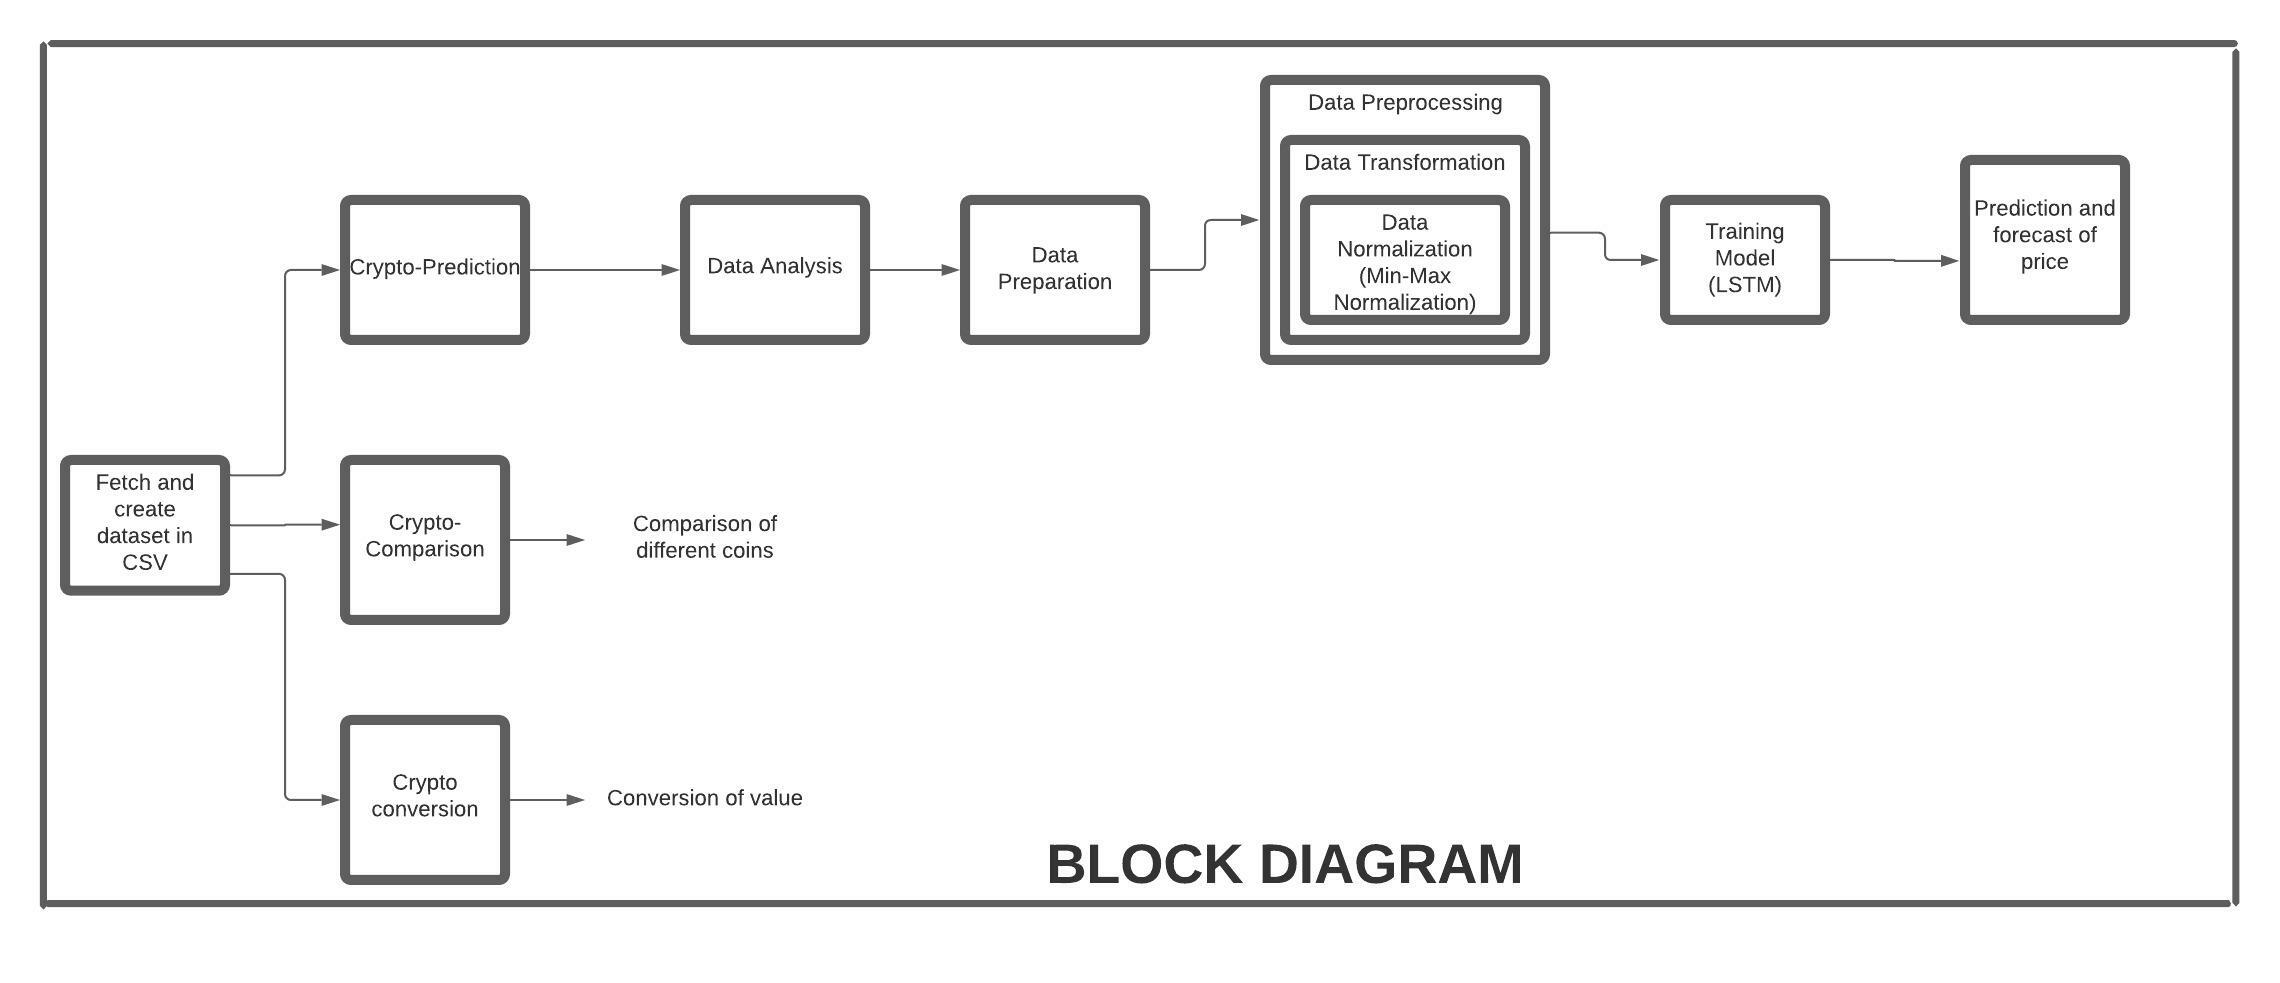
\includegraphics[width=6in,height=5in]{./Block diagram.jpeg}
\caption{Proposed Block diagram of application}
\end{figure}


\section{Summary}
In this chapter we discussed about history and future of cryptocurrency and we also see various terminologies used in cryptocurrency analysis and go through the various terminologies which are used in financial world for cryptocurrencies.  
\vfill
\hrule
%*************************Chapter 2************************
\chapter{Literature Survey}
In this chapter we will see the various studies and research conducted in order to identify the current scenarios and trends in cryptocurrency and also the study of prediction model using machine learnning.
%***********************************************************
\section{{\textit{A Novel Cryptocurrency Price Prediction \\model using GRU,LSTM and bi-LSTM machine \\learning algorithms.}}}
\\In this paper it is about prediction model based on machine learning for bitcoin price prediction, here they use the concept of LSTM, GRU and bi-LSTM.
This paper helps us to get knowlege about LSTM and its architecture \cite{paper1}.\\
%********************************************************
\section{{\textit{Machine learning models comparison for\\bitcoin price predict 2018.}}}\\
This paper proposes three types of recurrent neural network(RNN) algorithms used to predict the prices of three types of cryptocurrencies, namely Bitcoin
(BTC), Litecoin (LTC), and Ethereum (ETH). The models show excellent predictions depending on
the mean absolute percentage error (MAPE). Results obtained from these models show that the
gated recurrent unit (GRU) performed better in prediction for all types of cryptocurrency than the long short-term memory (LSTM) and bidirectional LSTM (bi-LSTM) models. Therefore, it can be
considered the best algorithm. GRU presents the most accurate prediction for LTC with MAPE
percentages of 0.2454\% , 0.8267\% , and 0.2116\% for BTC, ETH, and LTC, respectively. The bi-LSTM
algorithm presents the lowest prediction result compared with the other two algorithms as the
MAPE percentages are: 5.990\%, 6.85\%, and 2.332\% for BTC, ETH, and LTC, respectively. Overall, the
prediction models in this paper represent accurate results close to the actual prices of cryptocurrencies.
The importance of having these models is that they can have significant economic ramifications
by helping investors and traders to pinpoint cryptocurrency sales and purchasing. As a plan for
future work, a recommendation is made to investigate other factors that might affect the prices of
cryptocurrency market such as social media, tweets, and trading volume\cite{paper2}.\\
%*******************************************************
\section{\textit{Crypto-currency price prediction using decision tree and regression techniques 2018.}}\\
\\In this paper they have used several machine learning techniques and algorithms and compared the models with each other to get the best output. They believe that there work will help reduce the challenges and difficulties faced by people, who invest in cryptocurrencies. Moreover, the obtained results 
can play a major role in cryptocurrency portfolio management and in observing the fluctuations in the prices of constituents of cryptocurrency market. We have also compared our approach with similar state of the art works from the literature, where machine learning approaches are considered for predicting and forecasting the prices of these currencies. In the sequel, we have found that our best approach presents better and competitive results than the best works from the literature thereby advancing the state of the art. Using such prediction and forecasting methods, people can easily understand the trend and it would be even easier for 
them to trade in a difficult and challenging financial instrument like cryptocurrency.\cite{paper5}.\\

%*********************************************************
\\
\section{{\textit{Bitcoin price prediction using machine\\learning.2018}} }
\\This study is devoted to the problems of the short-term forecasting cryptocurrency time series using machine learning (ML) approach. Focus on studying of
the financial time series allows to analyze the methodological principles, including
the advantages and disadvantages of using ML algorithms. The 90-day time horizon
of the dynamics of the three most capitalized cryptocurrencies (Bitcoin, Ethereum,
Ripple) was estimated using the Binary Autoregressive Tree model (BART), Neural Networks (multilayer perceptron, MLP) and an ensemble of Classification and
Regression Trees models—Random Forest (RF) \cite{paper4}.\\
%*********************************************************
\\
\section{{\textit{Benchmarking of LSTM network.}}}\\
LSTM (Long Short-Term Memory) recurrent neural networks have been highly successful in a number of application areas. This technical report describes the use of the MNIST and UW3 databases for benchmarking LSTM networks and explores the effect of different architectural and
hyperparameter choices on performance. 
This report gives us a clear view of LSTM and its basic concepts which help a lot in project process \cite{paper7}.\\
%********************************************************
\\
\section{\textit{Convolutional LSTM network: A machine\\ learning approach for precipitation nowcasting.}}\\
\\According to these report the goal of precipitation nowcasting is to predict the future rainfall intensity in a local region over a relatively short period of time. Very few previous studies have
examined this crucial and challenging weather forecasting problem from the machine learning perspective. In this paper, we formulate precipitation nowcasting as a spatiotemporal sequence forecasting problem in which both the input and the
prediction target are spatiotemporal sequences. By extending the fully connected LSTM 

(FC-LSTM) to have convolutional structures in both the input-to-state and state-to-state transitions, we propose the convolutional LSTM (ConvLSTM) and use it to build an end-to-end trainable model for the precipitation nowcasting problem. Experiments show that our ConvLSTM network captures spatiotemporal correlations better and consistently outperforms FC-LSTM and the state-of-theart operational ROVER algorithm for precipitation nowcasting \cite{paper8}.\\
%********************************************************
\section{Summary}
In this chapter we discussed the best researches papers which we used for clear our concepts and use in order to achieve a clarity about use of  machine learning algorithms in various prediction models.
\vfill
\hrule
%*************************Chapter 3 ************************
\chapter{Problem Definition}
This chapter explains the need of prediction in  investment industry . It introduces the basic concepts of machine learning and problem definition which used in prediction model.It also explain the need of prediction model in functional sector for better investment and business growth.
\\
\section{Need of prediction in investment industry}
The investment industry is a subset of the financial services industry. It comprises all the participants that are instrumental in helping savers invest their money and helping spenders raise capital in financial markets.
\\
Just like a financial forecast gives businesses access to cohesive reports, allowing finance departments to establish business goals that are both realistic and feasible using the past data to make a way it will compare with the future.In the similar manner prediction in the field of cryptocurrency help both the small investors and the companies who help investors to invest there money.  
\\
\\
\section{Basic Concept of Machine Learning}
Machine learning is a method of data analysis that automates analytical model building. It is a branch of artificial intelligence based on the idea that systems can learn from data,

identify patterns and make decisions with minimal human intervention.
\begin{figure}[H]
\centering
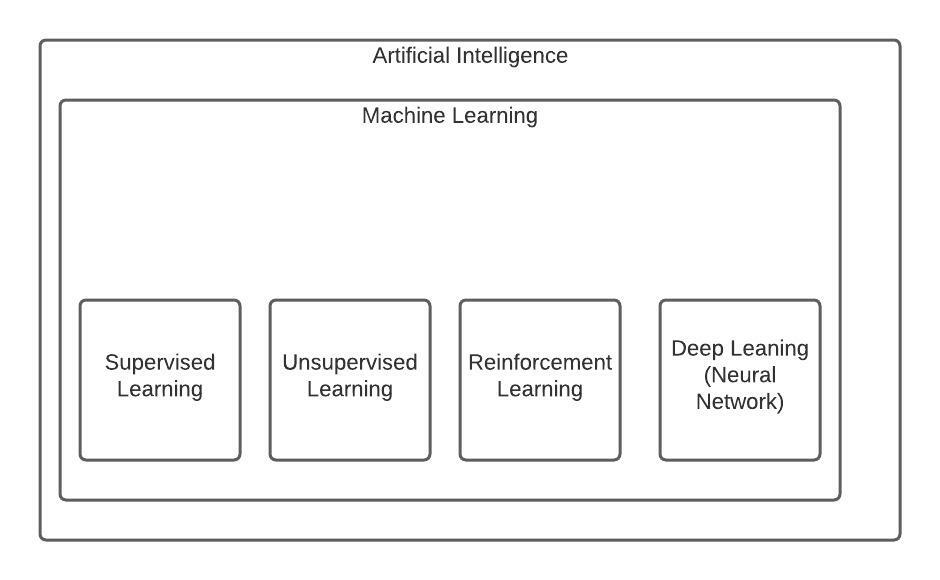
\includegraphics[width=5in,height=4in]{./MachineLearning.jpeg}
\caption{Proposed Block diagram of Machine Learning}
\end{figure}
\\
The above figure 3.1 shows the architecture of domains of Artificial Intelligence.\\
Machine learning is an important component of the growing field of data science. Through the use of statistical methods, algorithms are trained to make classifications or predictions.
\subsection{Use of Machine Learning in Predictive Models}
Predictive analytics and machine learning go hand-in-hand, as predictive models typically include a machine learning algorithm.These models are then made up of algorithms. The algorithms perform the data mining and statistical analysis, determining trends and patterns in data.
\\
Machine learning can increase the speed at which data is processed and analyzed, making it a useful technology for predictive analytic programs. Using machine learning, predictive analytic algorithms can train on even larger data sets and perform deeper analysis on multiple variables with minor changes in deployment.These models can be trained over 


time to respond to new data or values, delivering the results the business needs. Predictive modelling largely overlaps with the field of machine learning.
\\
There are two types of predictive models. They are Classification models, that predict class membership, and Regression models that predict a number. These models are then made up of algorithms. The algorithms perform the data mining and statistical analysis, determining trends and patterns in data. 
\\
The most widely used predictive models are:
\begin{itemize}
\item{Decision trees:}
Decision trees are a simple, but powerful form of multiple variable analysis. They are produced by algorithms that identify various ways of splitting data into branch-like segments. Decision trees partition data into subsets based on categories of input variables, helping you to understand someone’s path of decisions.
\item{Regression (linear and logistic):}Regression is one of the most popular methods in statistics. Regression analysis estimates relationships among variables, finding key patterns in large and diverse data sets and how they relate to each other.
\item{Neural networks:}Patterned after the operation of neuronsin the human brain, neural networks (also called artificial neural networks) are a variety of deep learning technologies. They’re typically used to solve complex pattern recognition problems – and are incredibly useful for analysing large data sets. They are great at handling nonlinear relationships in data and work well when certain variables are unknown.The best example of neural network concept is LSTM (Long short term memory).\cite{paper7}
\end{itemize}


\section{Summary}
In this chapter we introduced the concept of machine learning and see the types of methods used in predictive model for forecasting of cryptocurrency. Use of machine learning in predictive. 
\vfill
\hrule
%*****************************Chapter 4******************

\chapter{Analysis}
This chapter describes the project plan adopted and determines the requirement analysis. We have implemented the project on the basis of Agile model.
Where Agile process model is a software development approach based on iterative development.Agile methods break tasks into smaller iterations, or parts do not directly involve long term planning. The project scope and requirements are laid down at the beginning of the development process. 
\section{Project Plan}

\subsection{Project Plan for semester I}

The following Table 4.1 describes the project plan for semester I. It describes the various activities and accountability of the developers for the respective modules. Following are the major activities carried out in this plan :
\begin{itemize}
\item{Identifying software requirements.}
\item{Designing a architecture for proposed system.}
\item{Studying the necessary concepts , algorithms and technologies required to build the project}
\end{itemize}


\newpage
\begin{table} [htb]
\centering
\begin{tabular}{|p{1.2cm}|p{5cm}|p{2.5cm}|p{2.5cm}|p{3cm}| }\hline
\textbf{Phase} 	&\textbf{Activity}	&\textbf{Start Date}	&\textbf{End Date} &\textbf{Group Members}\\\hline\hline
1 &Selection of Project Topic	&12-08-2021 	&14-08-2021 &Team \\\hline
1 &System Requirement Specification(SRS) &14-08-2021 &22-08-2021 &Team\\\hline
1 &Design Prototype &23-08-2021 &28-08-2021 &Team\\\hline
1 &Mathematical Model &02-08-2021 &21-09-2011 & Vedant, Avinash \\\hline
1 &UML Diagram Prototype &12-09-2021 &20-09-2021 &Vedant , Ganesh \\\hline
1 &Project Problem Statement working &04-10--2021 &19-10-2021 & Team\\\hline
1 &UML Diagram in StarUML &05-10-2021 &22-10-2021 & Vedant , Ganesh \\\hline
1 &Software Requirement Specification &12-11-2021 &20-11-2021 &Team \\\hline
1 &Test Plan &01-12-2021 &15-12-2021 &Team \\\hline
\end{tabular}
\caption{Planner and Progress Report I for Prediction Model}
\label{tab:nnwork}
\end{table}

\subsection{Project Plan for semester II}
\hspace*{0.5in}The following Table 4.2 describes the project plan for semester II. It describes the various activities and accountability of the developers for the respective modules. Following are the major activities carried out in this plan :
\begin{itemize}
\item{Define Programming Standards.}
\item{Development of project in 3 Modules.}
\item{Formal Technical Review and Testing.}
\end{itemize}

\newpage
\begin{table} [htb]
%\centering
\begin{tabular}{|p{1.2cm}|p{5cm}|p{2.5cm}|p{2.5cm}|p{3cm}| }\hline
\textbf{Phase}	&\textbf{Activity}	&\textbf{Start Date}	&\textbf{End Date} &\textbf{Group Members}\\\hline\hline
2 &Defining Programming Standards	&10-10-2021 	& 15-10-2021 &Team \\\hline
2 &Development of Module No.1 & 08-12-2021 & 16-12 -2021 &Team\\\hline
2 &Development of Module No.2 & 01-04-2022 & 05-04 -2022 &Team\\\hline
2 &Development of Module No.3 & 10-04-2022 & 08-05 -2022 & Team \\\hline
2 &Formal Technical Review &02-04-2022 &10-05-2022 &Team \\\hline
2 &Testing and Bug Fixing  & 08-04-2022 &10-05-2022 &Team\\\hline

\end{tabular}
\caption{Planner and Progress Report II for Prediction,conversion and comparison models}
\label{tab:nnwork}
\end{table}

\section{Requirement Analysis}

\subsection{Necessary Functions}
\begin{itemize}
\item{Deliver a reusable piece of code.}
\item{Build all modules}
\item{Deployment of whole system as one.}
\end{itemize}


\section{Summary}
In this chapter we described the analyse details of the project plan for Semester I and Semester II .We also describes the necessary functions that we did in our process and the process to make Cryptocurrency research and analytical tool.
\vfill
\hrule
%*****************************Chapter5***************
\chapter{Design}
This chapter describes the Software Requirement Specification (SRS) to be implemented for our software. It also explains the architecture of the system and external interface requirements. We have also described the Risk assessment strategy and the Data Flow Diagram which explains the flow of the project.
\section{Software Requirement Specifications}
The Software Requirement Specification describes the scope of the project, operating environment, user characteristics, design and constraints. It also elaborates the system architecture of the cryptocurrency research and analytical tool.

\subsection{Project Scope}

For such type of project in which a concept like cryptocurrency is used where the popularity of cryptocurrencies are skyrocketing day by day and new businesses and platforms are coming up which are based on concept of cryptocurrency, for example platforms like Unocoin is one of the oldest cryptocurrency exchange platform in india, then companies like CoinSwitch Kuber now became India's newest cryto unicorn(companies having valued over 1 Billion dollor) .The number of cryptocurrency owner will increase to 200 million in comming years in india. Because of the growth of crypto in developed nations and mega companies wants to invest in it.
For such type of development in financial world requires a bedrock system to predict the future of such entities.
But due to the volatility of the cryptocurrency it becomes challenging to predict or forecast its future

value.But to the development in the field of data science and Artificial Intelligence which helps use in machine learning to create a predictive modeling.
\\For such type of model in which we use a concept like cryptocurrency we needed a perfect model to design the software for prediction for such type of model we use Agile model to design the software  which will be useful for high level of project. 
Agile model is a software development approach based on iterative development. Agile methods break tasks into smaller iterations, or parts do not directly involve long term planning. The project scope and requirements are laid down at the beginning of the development process.\\
Phases of Agile Model:
Following are the phases in the Agile model are as follows:\\
1. Requirements gathering\\
2. Design the requirements\\
3. Construction/ iteration\\
4. Testing/ Quality assurance\\
5. Deployment\\
6. Feedback\\
In this software we go through this phases first we gather the requirements for a prediction models like different research papers, then we design a proper flow for project then we construct a structure of software for coding then again we gather some more requirements again we correct the design again construct a new model then we conform weather the software is fulfilling the all requirement then after verification we start deployment , after deployment we again go to step 1 to check that it is fulfilling the problem statement or not. In this way using Agile model we completed our first model of prediction. 
A Predictive model has various of usability's like 
\begin{itemize}
\item{To forecast future outcomes.}
\item{It is a tool used in predictive analytical, a data mining technique that attempts to answer the question what might possibly happen in the future?.}
\item{Machine learning can increase the speed at which data is processed and analyzed,making it a useful technology for predictive analytical programs. Using ML,predictive analytical algorithms can train on even larger data sets and perform deeper analysis on multiple variables with minor changes in deployment.}

\end{itemize}
\\ 
\\
\newpage
Also the system is useful in many fields like:
\begin{itemize}
\item{Business}
\item{Investment}
\item{Education}
\item{Personal}
\end{itemize}
\subsection{Operating Environment}
We propose a predictive model to predict the future growth of the crypto using various data sets which are available on different platforms.A part from this we are also provide sub features like crypto-comparison which is able to compare data of two cryptocurries and suggest the user where to invest and crypto-conversion which help the user to check and compare the values.For now we choose to run the software on online platforms like Jupyter notebook for easy execution.

\subsection{User Classes and Characteristics}
The user who is going to operate the system should have phone or desktop from which he/she can see the analysis and prediction for his/her investment.
This software gives the user a power to predict the value , compare the value and convert the value for his/her investment.

\subsection{Design and Implementation Constraints}
Using mobile devices like phones, tablets, and laptops has a very different set of challenges. The issue which may user will face is speed issue because a training model takes huge time to process and as we know python is a slow language so it make take huge time to process.
User should have proper knowledge of graph and cryptocurrencies.
\\
Following are the merits of the design implementation :
\begin{itemize}
\item{\textbf{Portability:}  As it is python based code it is easy to transfer from one device to another.}
\item{\textbf{Easy to analyse:} It is simple and limited crypto data analysis makes to easy to analyse the data.  }

\item{\textbf{User-friendly:}  It is user-friendly, it has graphical representation.}
\end{itemize}

\section{System Architecture}
This Software has a very simple system architecture in which data is generated in CSV format from different data sources and fetch into the system then that data is Normalized and prepossessed to make it suitable for next steps then that data fetch by different models like prediction model for training process and then prediction. Similarly crypto-comparison model use the data for comparison and crypto-converter model will have that day of value in its data and on that bases it will give in how much coin we get how much coins.
\\
\begin{figure}[H]
\centering
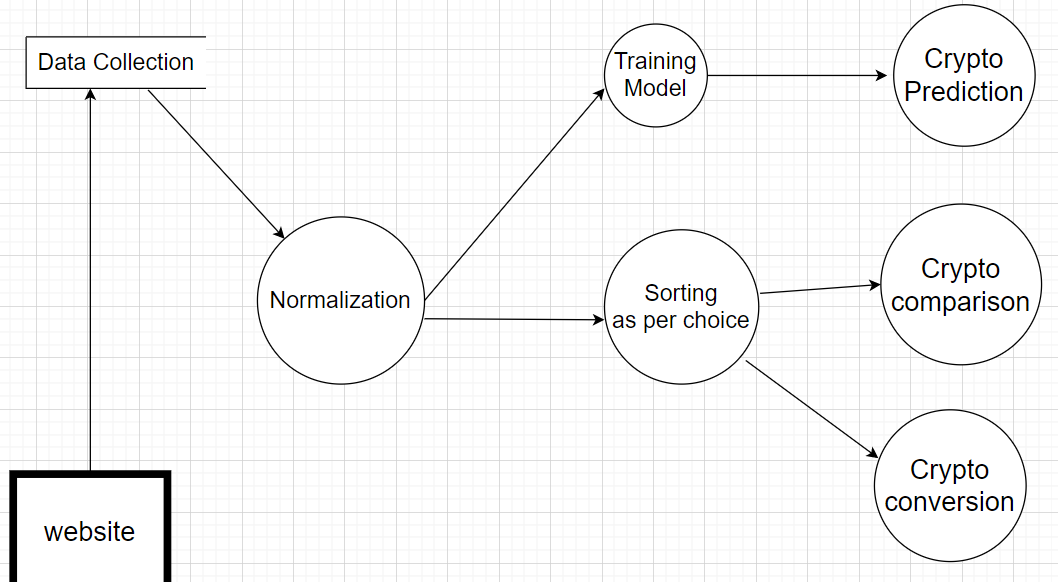
\includegraphics[width=5in,height=4in]{./System.png}
\caption{System Architecture}
\end{figure}
\\
\\ \\ \\
The above figure 5.1 represents the software architecture of the project where it represents all the processes of the project from data collection , training model , data normalization ,to the output of the system.

\section{External Interface Requirement}

\subsection{User Interfaces}

\begin{itemize}
\item{\textbf{Desktop Application:}  This is a desktop application using the desktop application the end user will be able to use all features in this tool provide. }

\end{itemize}

\subsection{Hardware Interfaces}
\begin{itemize}
\item{\textbf{Desktop Devices:}This Software is specially designed for a desktop system which require for which it requires less time to process the data.}
\item{\textbf{Mobile Devices:} This software can also be run on mobile devices but require a special application to run it.}
\item{\textbf{Internet:}  If user want to use the data source for the data set form outside of the system then he need a connect of internet to fetch the data from the database and user want to run the program online for easy processing. }
\end{itemize}


\section{Software System Attribute}
\begin{itemize}
\item{\textbf{Reliability:} This software can run on any device.if data source is out of system then Internet facility must be available for data set generation.}
\item{\textbf{Availability:} The application shall be available and running in a stable state at all times.}
\item{\textbf{Maintainability:}  This model requires very less maintainability and shall be require few updates for future features.}
\item{\textbf{Portability:}  This model is made using python which is system independent because they can be run on different platforms using an interpreter built specifically for the platform.}

\end{itemize}

\newpage
\section{Data Flow Diagram}
The Data Flow Diagram of the this model is as shown in Figure 5.2. The Data Flow Diagram explains the flow of information in the project that is it indicates from where information (data) is received (inputs) and where information is send (outputs) and this model is working.\\

\begin{figure}[H]
\centering
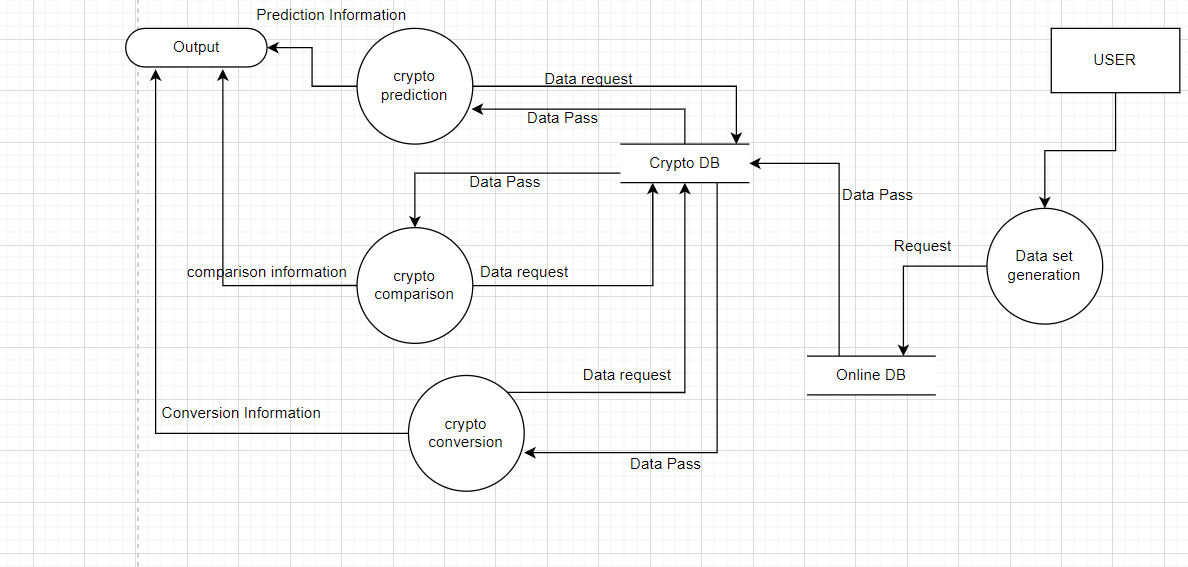
\includegraphics[width=6in,height=3in]{DataFlow .png}
\caption{Data Flow Diagram}
\end{figure}


\section{Summary}
 In this chapter we studied the operating environment, requirements,project scope, limitations, merits, system architecture, flow of system and the user classes and characteristics which describes the scope of the project. 
 \vfill
\hrule
%*****************************Chapter 6******************

\chapter{Modeling}
 This chapter includes the various modeling techniques which describes the various uses of the prediction model and Application. It also describes the functionality of the different features of the Model.

\section{Use Case Diagram}
 A use case diagram is a type of behavioral diagram defined by the UML created from a use case analysis. Its purpose is to present a graphical overview of the functionality provided by a system in terms of actors, their goals represented as use case and any dependencies between those use cases.
 In the figure 6.1 shows the user interation with software.\\
Four modeling elements make up the use case diagram these are:\\
\begin{itemize}
\item{\textbf{Actors:} Actors refer to a type of users, users are people who use the system. In this case investor is the users of the  end application}
\item{\textbf{Use cases:} A use case defines behavioral features of a system. Each use case is named using a verb phrase that express a goal of the system. The name may appear inside or outside the ellipse.In this case the goal is to predict , compare and convert the values.}
\item{\textbf{Associations:} An association is a relationship between an actor and a use case. The relationship is represented by a line between an actor and a use case.In this case user request the system to forecast the values.}

\item{\textbf{The include relationship:} It is analogous to a call between objects. One use case requires some type of behavior which is fully defined in  another use case.}
\end{itemize}
\begin{figure}[H]
\centering
\includegraphics[width=5in,height=5.5in]{./Use case diagram.png}
\caption{Use Case Diagram}
\end{figure}
In the above figure 6.1 shows the use case diagram that is the interaction of the user with system.

\newpage
\section{Sequence Diagram}
The sequence diagram is used primarily to show the interactions between objects in the sequential order that those interactions occur. Developers typically think sequence diagrams were meant exclusively for them. However, an organization's business staff can find sequence diagrams useful to communicate how the business currently works by showing how various business objects interact.Sequence diagrams illustrate how objects interact with each other. They focus on message sequences, that is, how messages are sent and received between a number of objects. The main purpose of sequence diagram is to show the order of events between the parts of system that are involved in particular interaction.\\
The basic element of sequence diagram is collection of participants, that is, the parts of the system that interact with each other during the sequence. The participants are arranged horizontally with no two participants overlapping each other. in Figure 6.2 investor applications are some examples of participants. A message is communication between objects that conveys information with the expectation that action will be taken. An event is any point in an interaction where something occurs. Message can flow in whatever direction makes sense for the required interaction from left to right, right to left, or even back to the Message Caller itself.

\begin{figure}[H]
\centering
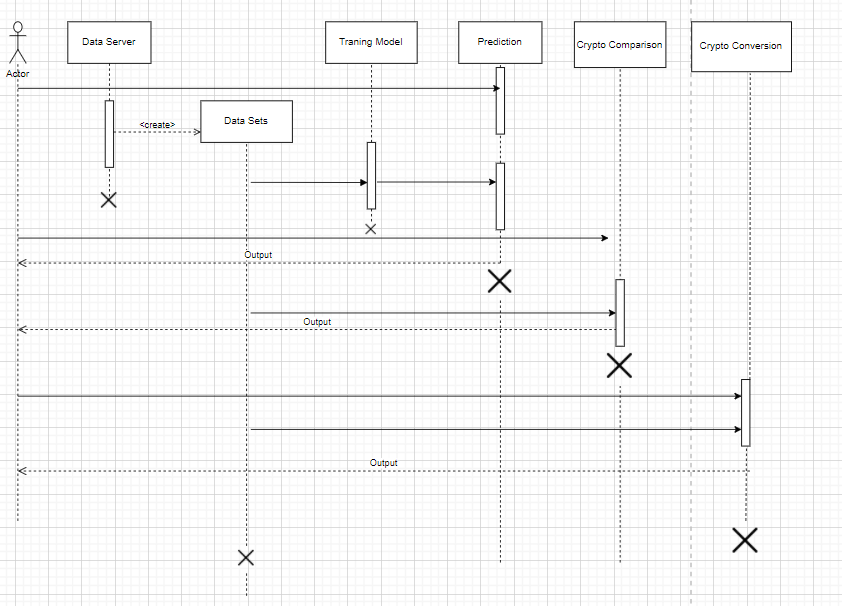
\includegraphics[width=5in,height=3.3in]{./Sequence Dig.png}
\caption{Sequence Diagram}
\end{figure}


\newpage
\section{Data Flow Diagram}
A data-flow diagram is a way of representing a flow of data through a process or a system. The DFD also provides information about the outputs and inputs of each entity and the process itself. A data-flow diagram has no control flow there are no decision rules and no loops.
A data flow diagram shows the way information flows through a process or system. It includes data inputs and outputs, data stores, and the various sub processes the data moves through. We can use these diagrams to map out an existing system and make it better or to plan out a new system for implementation.

\begin{figure}[H]
\centering
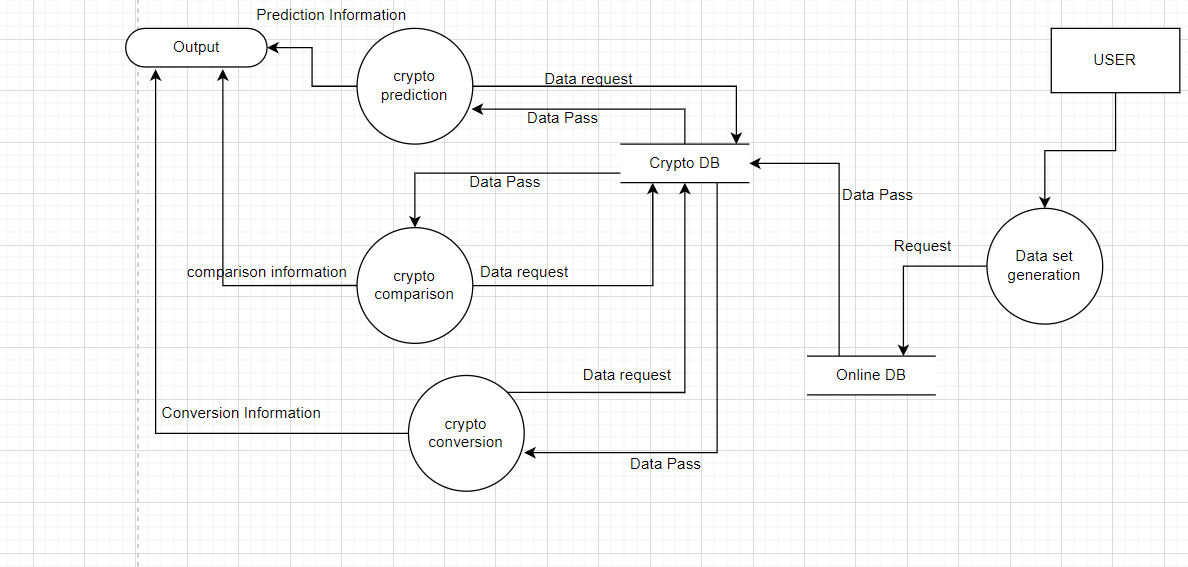
\includegraphics[width=5in,height=3.3in]{./Data Flow Diagram.png}
\caption{Data Flow Diagram}
\end{figure}

\newpage
\section{Deployment Diagram}
The deployment diagram depicts the runtime architecture of devices, execution environments and artifacts that reside in this architecture. It is the ultimate physical description of the system topology, describing the structure of the hardware units and the software executes on each unit. The deployment diagram shows how a system will be physically deployed in the hardware environment. Its purpose is to show where the different components of the system will physically run and how they will communicate with each other.

\begin{figure}[H]
\centering
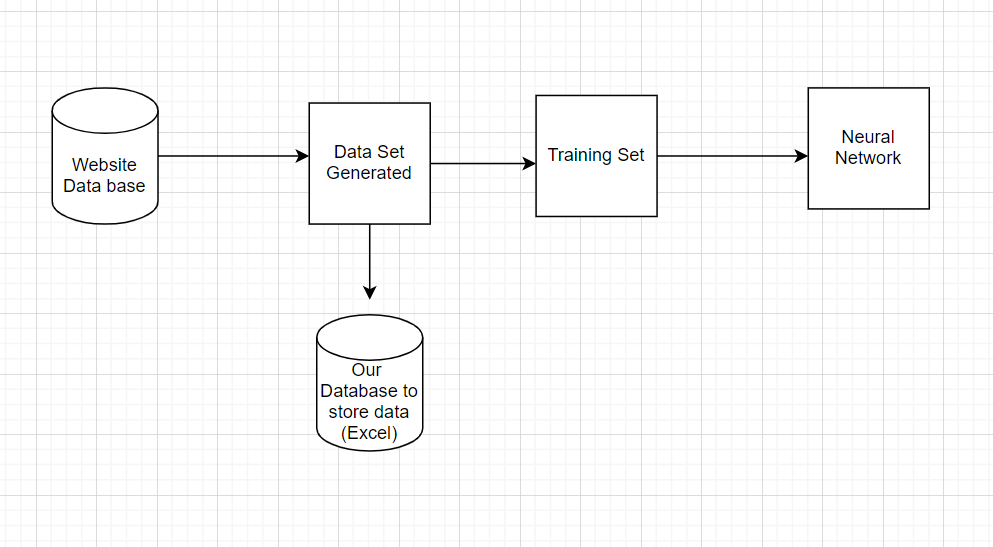
\includegraphics[width=5in,height=3.3in]{./Deployment.png}
\caption{Deployment Diagram}
\end{figure}

\begin{figure}[H]
\centering
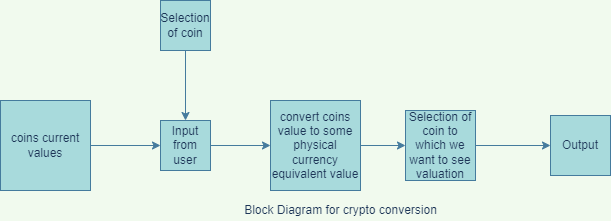
\includegraphics[width=7in,height=4in]{./Cryptoconvertor.png}
\caption{Block Diagram for cryptoconvertor}
\end{figure}




\section{Summary}
Thus we saw the various modeling techniques like use case diagram,sequence diagram,data flow diagram,deployment diagram used for the design of Cryptocurrency Research and Analytical Tool.
\vfill
\hrule
%*****************************Chapter 7******************
\chapter{Proposed System Model}
This chapter consists of the various implementation details and snapshots of the Cryptocurrency Prediction Tool developed using the Machine Learning .

\section{Implementation Details}
This section describes the various features of the Prediction model and also describes the implementation methods. Following are some of the features explained with their implementation details:\\
\begin{itemize}

\item{\textbf{Prediction Model:}}
Predictive modelling uses statistics to predict outcomes. Most often the event one wants to predict is in the future, but predictive modelling can be applied to any type of unknown event, regardless of when it occurred.

\item{\textbf{Data Analysis:}}
Data analysis is a process of inspecting, cleansing, transforming, and modelling data with the goal of discovering useful information, informing conclusions, and supporting decision-making. 

\item{\textbf{Normalization:}} Normalization is a technique often applied as part of data preparation for machine learning. The goal of normalization is to change the values of numeric columns in the dataset to a common scale, without distorting differences in the ranges of
values.

\item{\textbf{Data Preprocessing:}}
Data preprocessing can refer to manipulation or dropping of data before it is used in order to ensure or enhance performance, and is

an important step in the data mining process. The phrase "garbage in, garbage out" is particularly applicable to data mining and machine learning projects.

\item{\textbf{Training Model:}}
A training model is a dataset that is used to train an ML algorithm. It consists of the sample output data and the corresponding sets of input data that have an influence on the output. The training model is used to run the input data through the algorithm to correlate the processed output against the sample output.

\item{\textbf{Recurrent Neural Network (RNN):}}
It is a type of neural network where the output from previous step are fed as input to the current step.
In other neural networks all the inputs and outputs are independent of each other , but in case when we need predictions we need previous data , Hence there is a need to remember the previous data.
RNN which solves this issue of previous data with the help of a hidden layer. The main and most important feature of RNN is hidden state which remembers some sequence.
RNN have a "memory" which remembers all information about what has been calculated.
It uses the same parameters for each input as it performs the same task on all the inputs or hidden layers to produce output.This reduces the complexity of parameters.

\begin{figure}[H]
\centering
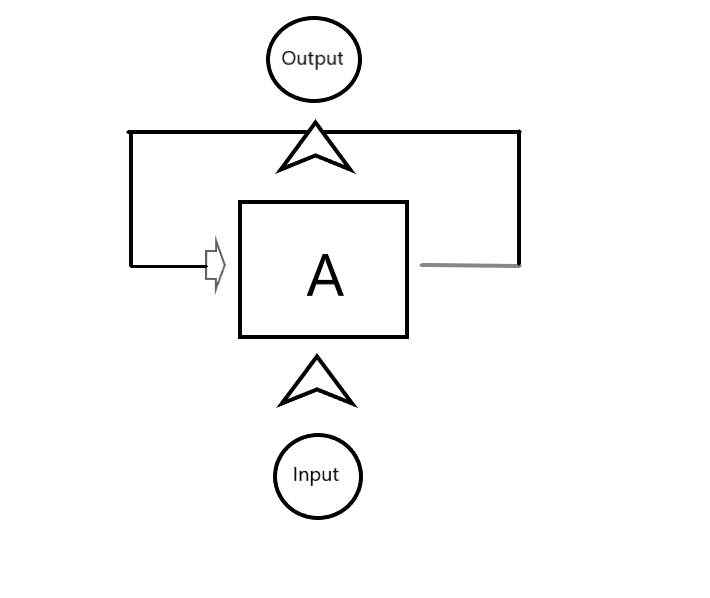
\includegraphics[width=5in,height=3in]{./RNN.png}
\caption{RNN}
\end{figure}

\section{Activation function}\\
The activation functions is a non-linear transformation that we do over the input before sending it to the next layer of neurons or finding it as output.
\\
An activation function is a function that is added into an artificial neural network in order to help the network learn complex patterns in the data. 
The purpose of the activation function is to introduce non-linearity into the output of a neuron. We know, neural network has neurons that work in correspondence of weight, bias and their respective activation function.
\\
\item{\textbf{Types of Activation functions:}}\\
1. Sigmoid function.\\
2. Leaky ReLU\\
3. tanh\\
4. Maxout\\
5. ReLU\\
6. ELU\\
\item{\textbf{Tanh function:}}\\
1. Tanh is a non linear activation function.\\
2. It regulates the      values flowing through the network, maintaining the values between -1 and 1.\\
3. Use of tanh function so that when input is enormous it will squish all values between -1 and 1.\\
4. It is symmetric about the origin, where the inputs would be normalized and they are more likely to prouduce outputs.\\

\begin{figure}[H]
\centering
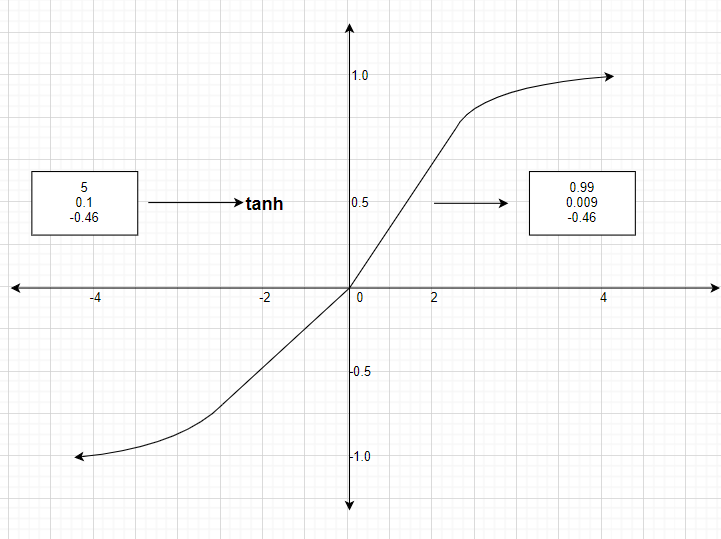
\includegraphics[width=5in,height=3in]{./Tanh.png}
\caption{Tanh function graph}
\end{figure}

\item{\textbf{Sigmoid function ($\sigma$):}}\\
1. It is a non linear activation function.\\
2. Like tanh It also regulates the values flowing through the network, maintaining the values between -1 and 1.\\
3.It helps the forget gate to update or to forget the data for long term memory.\\
4. If the result is in 0 the information is considered forgotten is considered forgotten and if the value is 1 it is stay.\\
5. This will help the network to learn which data can be forgotten and which data is important.\\

\begin{figure}[H]
\centering
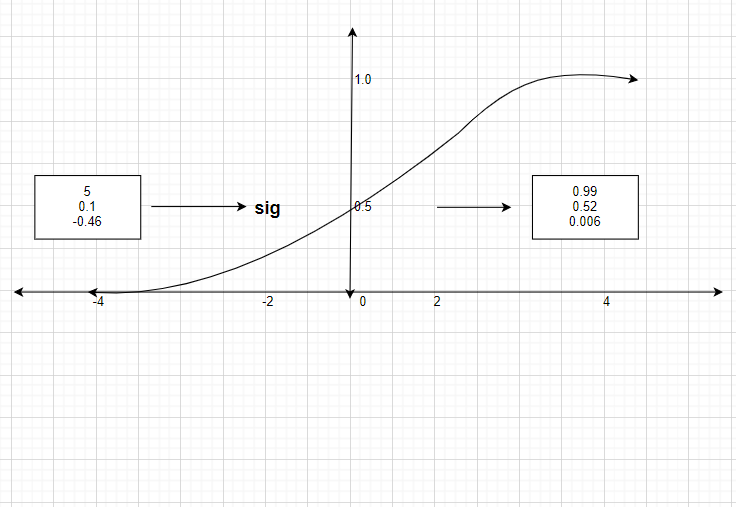
\includegraphics[width=5in,height=3in]{./sig.png}
\caption{sigmoid function graph}
\end{figure}

\item{\textbf{Architecture of LSTM:}}
It works by using special gates to allow each LSTM layer to take
information from both previous layers and the current layer.
The data goes through multiple gates (like forget gate, input
gate, etc.) and various activation functions (like the tanh
function) and is passed through the LSTM cells.\\

\item{\textbf{LSTM:Forget gate operation}}\\ 

In a cell of the LSTM network, the first step is to decide whether we should keep the information from the previous timestamp or forget it. Here is the equation for forget gate.Later, a sigmoid function is applied over it. That will make ft a number between 0 and 1. This ft is later multiplied with the cell state of the previous timestamp as shown below.If ft is 0 then the network will forget everything and if the value of ft is 1 it will forget nothing.
A forget gate is responsible for removing information from the cell state. The information that is no longer required for the LSTM to understand things or the information that is of less importance is removed via multiplication of a filter. This is required for optimizing the performance of the LSTM network.
This gate takes in two inputs; $h_{t-1}$ and $x_t$. $h_{t-1}$ is the hidden state from the previous cell or the output of the previous cell and $x_t$ is the input at that particular time step. The given inputs are multiplied 

by the weight matrices and a bias is added. Following this, the sigmoid function is applied to this value. The sigmoid function outputs a vector, with values ranging from 0 to 1, corresponding to each number in the cell state. Basically, the sigmoid function is responsible for deciding which values to keep and which to discard. If a ‘0’ is output for a particular value in the cell state, it means that the forget gate wants the cell state to forget that piece of information completely. Similarly, a ‘1’ means that the forget gate wants to remember that entire piece of information. This vector output from the sigmoid function is multiplied to the cell state.\\
\\
The equation for forget gate:\\


$f_{t}=\sigma(W_{t}.[h_{t-1},X_{t}]+b_{t})$
\\

where:\\
$t=timestep $\\
$\sigma=sigmoid function $
$f_{t}=forget gate at t $ \\
$W_{t}=weight matrix of forget gate $ \\
$b_{t}=condition bias at t $  \\ 
$X_{t}=current input $  \\
$h_{t-1}=Previous hidden state data $
\\
\begin{figure}[H]
\centering
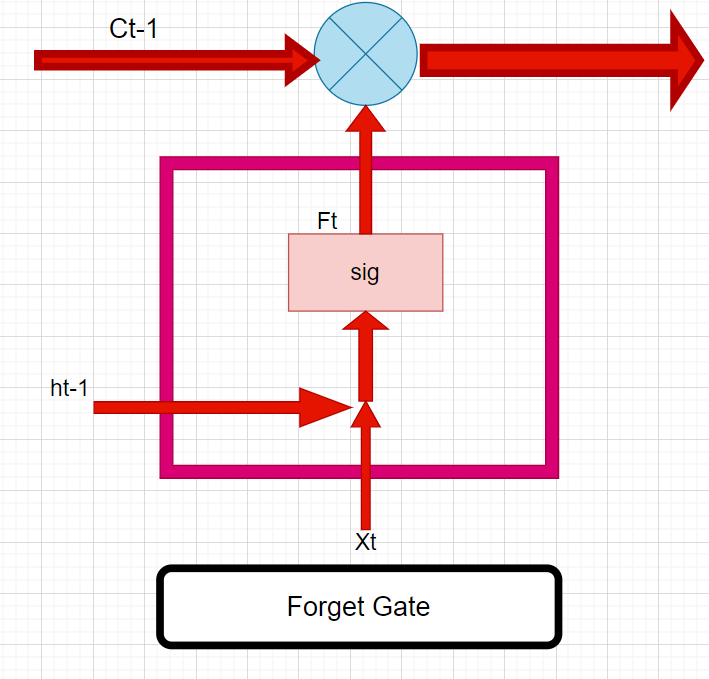
\includegraphics[width=5in,height=3in]{./Forget Gate.png}
\caption{Forget gate }
\end{figure}

\item{\textbf{LSTM:Input Gate operation}}\\
The input gate is responsible for the addition of information to the cell state. This addition of information is basically three-step process as seen from the diagram above.
Regulating what values need to be added to the cell state by involving a sigmoid function. This is basically very similar to the forget gate and acts as a filter for all the information from $h_{t-1}$ and $x_t$.
Creating a vector containing all possible values that can be added (as perceived from $h_{t-1}$ and $x_t$) to the cell state. This is done using the tanh function, which outputs values from -1 to +1.  
Multiplying the value of the regulatory filter (the sigmoid gate) to the created vector (the tanh function) and then adding this useful information to the cell state via addition operation.
 

Once this three-step process is done with, we ensure that only that information is added to the cell state that is important and is not redundant.\\
The equation we get from input gate:\\
\\
\\
$i_{t}=\sigma(W_{t}.[h_{t-1},X_{t}]+b_{t})$\\

\newpage
where:\\
$t=time step $\\
$\sigma=sigmoid function $\\
$i_{t}=input gate at t $ \\
$W_{t}=weight matrix of input gate $ \\
$b_{t}=condition bias at t $  \\ 
$X_{t}=current input $\\
$h_{t-1}=Previous hidden state $
\\
\\
\begin{figure}[H]
\centering
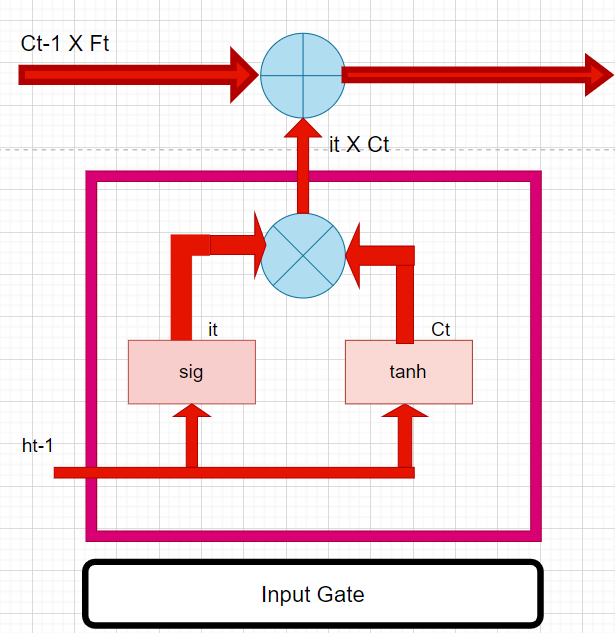
\includegraphics[width=5in,height=3in]{./Input Gate.png}
\caption{Input gate}
\end{figure}

\item{\textbf{LSTM:Cell state operation}} \\


The equation that we get is:\\
\\
$C_{t}=tanh(W_{c}.[h_{t-1},X_{t}]+b_{c})$
\\

\newpage
where:\\
$t=timestep $\\
$tanh=tan function $
$C_{t}=Cell state at t $ \\
$W_{c}=weight matrix of cell state $ \\
$b_{c}=condition bias at t $  \\ 
$X_{t}=current input $\\
$h_{t-1}=Previous hidden state $
\\
\\
\begin{figure}[H]
\centering
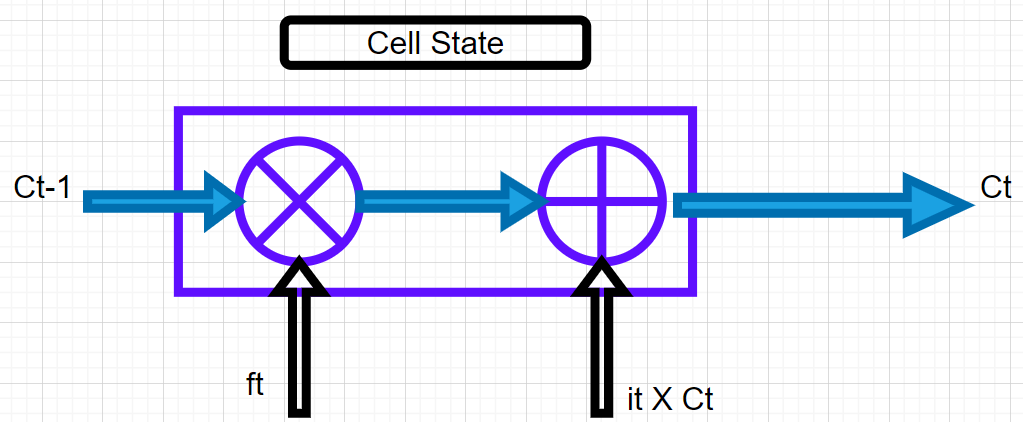
\includegraphics[width=5in,height=3in]{./Cell State.png}
\caption{Cell State}
\end{figure}

\item{\textbf{LSTM:Output gate operation}} \\
This job of selecting useful information from the current cell state and showing it out as an output is done via the output gate.The functioning of an output gate can again be broken down to three steps:

Creating a vector after applying tanh function to the cell state, thereby scaling the values to the range -1 to +1.
Making a filter using the values of $h_{t-1}$ and $x_t$, such that it can regulate the values that need to be output from the vector created above. This filter again employs a sigmoid function.
Multiplying the value of this regulatory filter to the vector created in step 1, and sending it out as a output and also to the hidden state of the next cell.

\newline
The equation that we get is:\\
$O_{t}=\sigma(W_{o}.[h_{t-1},X_{t}]+b_{o})$ \\ 
$h_{t}=O_{t} * tanh(C_{t}) $\\
\\
\\
where: \\
$t=timestep $\\
$O_{t}=output gate at t $ \\
$W_{o}=weight matrix of output gate $ \\
$b_{o}=bias vector w.r.t W_{o} $  \\ 
$h_{t}=LSTM output $  \\
\\

\begin{figure}[H]
\centering
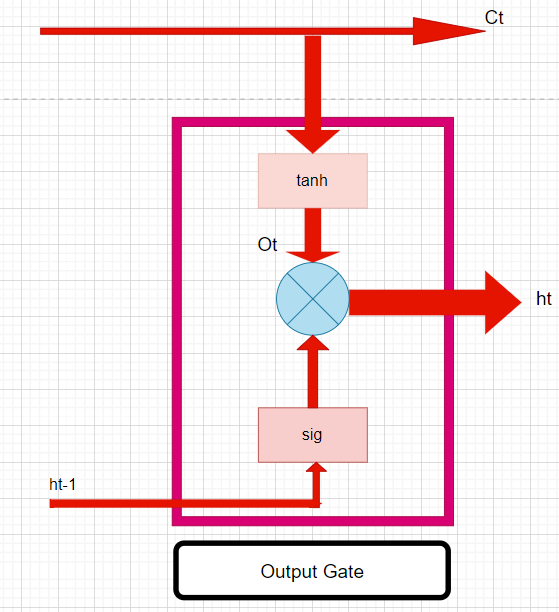
\includegraphics[width=5in,height=3in]{./Output Gate.png}
\caption{Output Gate}
\end{figure}

The main advantage of this is that it allows each LSTM cell to
remember patterns for a certain amount of time. The thing to be
noted is that LSTM can remember important information and at
the same time forget irrelevant information.a LSTM layer followed by 20 percent Dropout
layer and a Dense layer with linear activation function. The LSTM
architectures is shown below:

\newline
\end{itemize}
\begin{figure}[H]
\centering
\includegraphics[width=5in,height=3in]{./LSTM Dig.png}
\caption{LSTM}
\end{figure}

\section{Results}
\item{\textbf{ Data Set Graphical Analysis}\\

\begin{figure}[H]
\centering
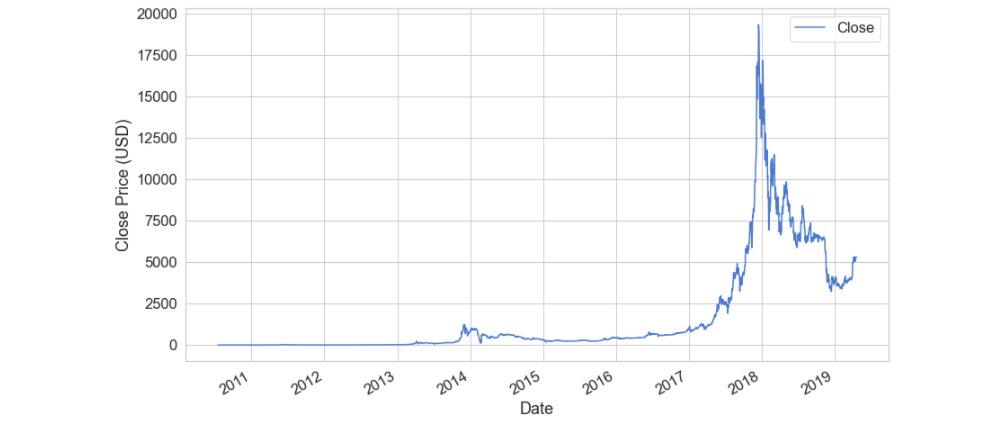
\includegraphics[width=5in,height=3in]{./Data Base.jpeg}
\caption{Data Set Graphical Analysis}
\end{figure}

\newline
In the above graph figure 7.9 it is actually the output of the software which representing the analysis of the data in data set.
\\
\item{\textbf{Data Loss After Normalization}\\

\begin{figure}[H]
\centering
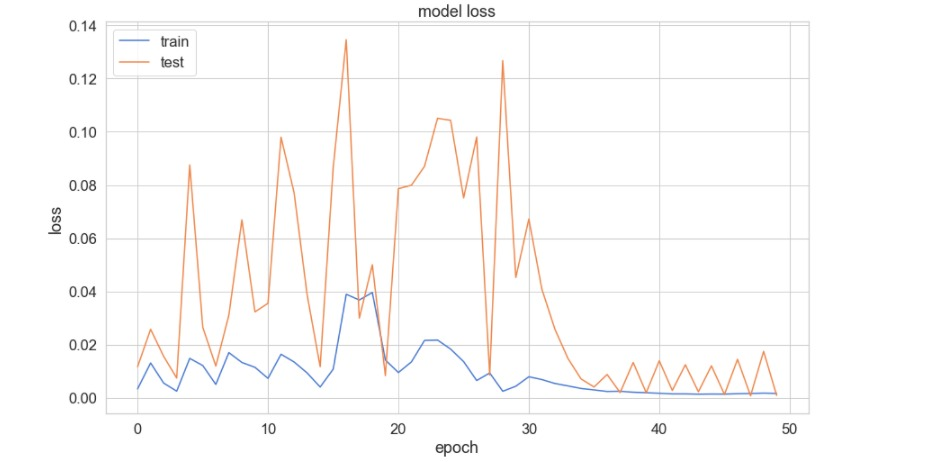
\includegraphics[width=5in,height=3in]{./Data Normalization.jpeg}
\caption{Data Loss After Normalization Representation}
\end{figure}
In the above graph figure 7.10 it is the output of the software which representing the data loss after Normalization.
\\
\\
\item{\textbf{Mean Absolute Error}\\ Mean Absolute Error is a model evaluation metric used with regression models. The mean absolute error of a model with respect to a test set is the mean of the absolute values of the individual prediction errors on over all instances in the test set.
Find all of your absolute errors, xi – x. Add them all up. Divide by the number of errors. For example, if you had 10 measurements, divide by 10.
mean absolute error is a measure of errors between paired observations expressing the same phenomenon. Examples of Y versus X include comparisons of predicted versus observed, subsequent time versus initial time, and one technique of measurement versus an alternative technique of measurement.

\newpage
The equation for Mean Square Error:\\


$MSE=1/n \sum_{n=1}^{n} (Y_{i}-\hat{Y_{i}})$
\\
$where:$\\
$MSE=Mean Square Error $\\
$n=number of data points $\\
$Y_{i}=observed   values$\\
$\hat{Y_{i}}=predicted values$ \\
\item{\textbf{Root Mean Square Error}\\ Root mean squared error (RMSE) is the square root of the mean of the square of all of the error. The use of RMSE is very common, and it is considered an excellent general-purpose error metric for numerical predictions.
\\
For every data point, you take the distance vertically from the point to the corresponding y value on the curve fit (the error), and square the value.
\\
So if we were to run a model with different parameters/independent variables, model with lower RMSE will be deemed better.
\\
Root Mean square error is always positive.
\\
If we have two models and the model which has lower MSE which near to 0 is considered as better.
\\
The equation for Mean Square Error:\\


$RMSE=\sqrt{1/n \sum_{n=1}^{n} (Y_{i}-\hat{Y_{i}})^2$}
\\

$where:$
\\
\\
$RMSE=Root Mean Square Error $
\\
\\
$n=number of data points $
\\
\\
$Y_{i}=observed   values$
\\
\\
$\hat{Y_{i}}=predicted values$ 
\\

\newpage
\textbf{Why we use MAE instead of RMSE?}\\ \\
The reason behind choosing MAE over Root Mean Square Error(RMSE)is that MAE is more interpretable. RMSE does not describe average error alone and hence is much more difficult to understand. Since we want the model to be readily explained even to the non technical audience, MAE looks like a better choice.
\\
\\
\begin{figure}[H]
\centering
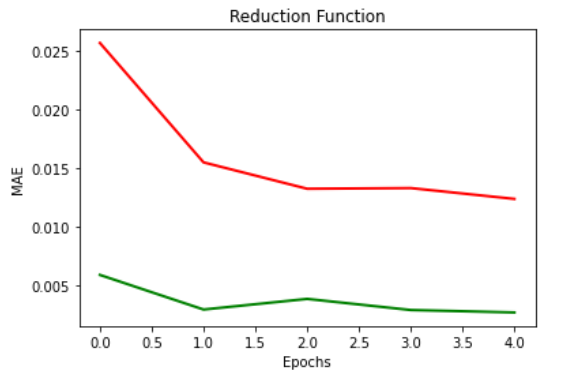
\includegraphics[width=6in,height=6in]{./Reduction.png}
\end{figure}

\\
\newpage
\item{\textbf{Data Prediction}\\
\\
So when MSE value obtained looks good.Finally we plot the actual and predicted prices
\begin{figure}[H]
\centering
\includegraphics[width=5in,height=3in]{./Prediction.jpeg}
\caption{Price Prediction}
\end{figure}
\\ \\
In the above graph figure 7.11 it is the output of the software which representing the prediction of the cryptocurrency upto 160 days from the last date of the data.\\

In this way we create a model which predicts the value of cryptocurrency using its past data.

\clearpage
\section{Crypto-Comparison}\\

In this model we find out the growth percentage of the cryprtocurrency with the help of their growth percentage and growth values.

Where the x-axis representing growth percentage and y-axis representing growth value.

In this we take two array list which contain growth percentage and growth value.

Where we removes the NULL value using the $remove_nan_targets.items()$ function.
\begin{figure}[H]
\centering
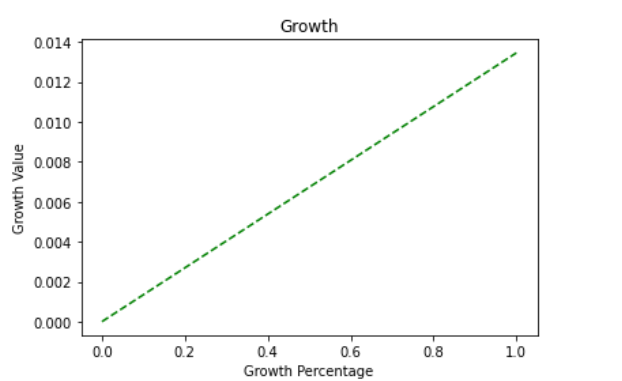
\includegraphics[width=5in,height=3in]{./growth.png}
\caption{Graph Representing growth Rate }
\end{figure}

 The above graph represents the growth of cryptocurrencies with its coordinates.

\\
\\
\clearpage
\section{Crypto-Coversion}\\
\\
It is a GUI based model in which user can get the information of how much he get the other coin in exchange of his coin.

Below is the block diagram of the model which is explaining that how user will get the interface.
For prototype we use Tkinter which is one of the GUI tool in python to create this model.
\\
\begin{figure}[H]
\centering
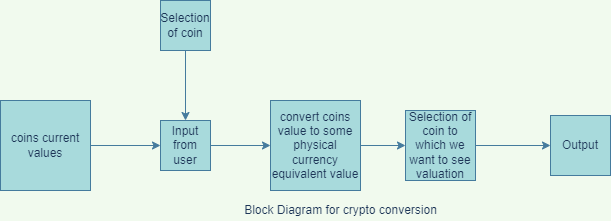
\includegraphics[width=4in,height=3in]{./Cryptoconvertor.png}
\caption{Block Diagram of Crypto-Convertor }
\end{figure}
\\
\section{Summary}
In this chapter we discussed the implementation,Architecture and various gates in LSTM which is one of the most vital part of the model and also the implementation of various features included its results of the model.\cite{paper1,paper3,paper6} 
\vfill
\hrule
%*****************************Chapter 8******************

\chapter{Testing}
This chapter includes the details of Formal Technical Review meetings and describes the process carried during the review process. It also includes the Test Plan adopted for testing the software.
\section{Formal Technical Review}
Formal Technical Reviews and Inspections of documents or software are performed to identify and
remove defects. The Formal Technical Review of our project was carried at regular intervals in the form of stand-up meetings and brainstorming sessions conducted in presence of Mr. Sandip Kahate. The process included verification of the code which was developed for the review process ,the code review  checklist template is as follows:

\begin{itemize}
\item{{Is the code well-structured , consistent in style and consistently formatted?}}
\item{{Are all variables properly defined with meaningful,consistent and clear names?}}
\item{{Does the code consist of comments ?}}
\item{{Is the code error free?}}
\item{{Does software is able to perform its application of prediction?}}
\end{itemize}

\\
\newpage
\section{Test Model}
 Type of testing we use in our project:
 \\
We use Debugging oriented testing:
\begin{itemize}

\item{{This is a type of testing in which developer were expected to debug the product while building it.}}
\item{{Tests were not documented and heuristically conducted.}}
\item{{Testing was considered to check correct working of implementation \\(positives testing.)}}
\end{itemize}
\\
We also use the White Box Testing for our model:
\\It is a method of software testing that tests internal structures or workings of an application, as opposed to its functionality. In white-box testing an internal perspective of the system, as well as programming skills, are used to design test cases.

\subsection{Prediction Model Testing}In this model we tested various elements like:
\begin{itemize}

\item{{Data set generation}}
\item{{Scaling and Normalization}}
\item{{Training and Testing Set}}
\item{{Working of LSTM}}
\end{itemize}

\subsection{Comparison Model Testing} In this model we tested various elements like:
\begin{itemize}
\item{{Data set fetching}}
\item{{Array List creation}}
\end{itemize}

\subsection{Value Conversion Model Testing}
\begin{itemize}
\item{{Testing GUI}}
\end{itemize}

\section{Test Cases}

\begin{tabular}{|p{1.2cm}|p{5cm}|p{2.5cm}|p{2.5cm}|p{3cm}| }\hline
\textbf{S. No} 	&\textbf{Module Tested}	&\textbf{Actual Result}	&\textbf{Expected Result} &\textbf{Decision}\\\hline\hline
1 & Data fetching with the use of API 	& Data from website show in csv format & With the use of API data get fetch from website and store as csv format & Pass \\\hline
2 & Data Scaling And Normalization&The range of data is change &scaling-the range of data is change, Normalization -data get distributed&Pass\\\hline
3 &Training Set And Testing Set & Testing- 20 percent Training-80 percent &Data get divided into training and testing set with the use of scikit-lear &Pass\\\hline
4 &Predicted coordinates for graph &Give coordinates&Give coordinates for predicted values &Pass \\\hline
5 &Creation of growth value and growth percentage coordinates&Coordinates for growth & Give coordinates for growth graph&Pass\\\hline
6 &Selection coin &Successfully working &GUI for selection of coin & Pass \\\hline
7 &Input to the conversion model& Value we want to convert & how much we get other coin in it &Pass\\\hline
\end{tabular}

\\
\\

\section{Summary}
In this chapter we have described the formal technical reviews and the outcome of the model. We have described the Test Plan which was successfully carried out at regular development phases.\\
\vfill
\hrule
%*******************t**********Chapter 9******************
\chapter{Technical Specifications}
\hspace*{0.5in}In this chapter we will discuss the advantages and limitations of the Software. We will also go through the applications and have a brief study about the technical requirements.
\section{Advantages}
This prediction model aims to determine the future movement of the cryptocurrencies. The accurate prediction of crypto price will lead to more profit investors can make.
Prediction analytic provides valuable information for decision making.This enables investors to take advantage of future trends and , at the same time, respond to challenges before they occur.
\\Following are some more advantages of this tool to users:
\begin{itemize}
\item{{Fast Prediction}}
\item{{Available to ever investor}}
\item{{No need to wast time on huge data of cryptocurrency}}
\item{{Focus on limited coins}}
\item{{Feature of comparison help user to compare on run time.}}
\item{{Feature like crypto-conversion help user to convert value at run time.}}
\end{itemize}

\section{Limitations}
Just like a coin ever object has two sides pros and cons, similarly this project has also has two sides one side where common investor get a chance to predict , analyse , compare and convert the crypto without wasting his time to analyse all 8000 cryptocurrencies.
But on the other hand this prediction also has some limitations like data incomplete, if data we are using from a surveys,then people don't always provide accurate information. Data collection from different sources can vary in quality and format.It is possible that prediction and actual future value has a great difference due to volatility of crypto.This model works on training process which may take huge time to process depends on users system.

\section{Applications}
The Prediction model can be used in following areas:
\begin{itemize}
\item{Used in business who want to invest into crypto}
\item{Useful for investor who want to invest his hard earn money in the future currency }
\item{With the help of this model Students can take the idea of prediction model and machine learning.}
\end{itemize}
\subsection{Hardware Requirements}
\begin{itemize}
\item{Intel i5 Processor}
\item{2GB RAM for application development}
\item{Internet Connection}
\item{GPU like GTx 600 series}
\end{itemize}
\subsection{Software Requirements}
\begin{itemize}
\item{Python}
\item{Google collab}
\item{jupyter notebook}
\end{itemize}

\subsection{IDE Used}
\begin{itemize}
\item{Google collab}
\item{jupyter notebook}
\item{pycharm}
\end{itemize}

\subsection{Software Domains}
\begin{itemize}
\item{Python}
\item{Artificial Intelligence}
\item{Machine Learning}
\item{Data Mining}
\item{Data Analytic}
\item{Tkinter}
\end{itemize}

\section{Summary}
In this chapter we were made aware of the various advantages of the our tool and also the limitations of the project. We also saw the hardware, software, domain and IDE requirements of the project.
\cite{paper2}

\vfill
\hrule
%***************************Chapter 10**************
\chapter{Future Scope}
\hspace{0.5in}This project is useful on multiple platforms in this digital
learning age and has a bright future. Although we tried to deliver a project that meets the present requirements of the prediction and analysis application but there are endless future possibilities. Some are listed below:

\\
\begin{itemize}
\item{We visualize this tool will works on every gadget because in today's world investor wants current value to invest.}
\item{We visualize this tool will even work on wearable devices like smart glasses , smart bracelet or smart watches which we can make possible with the use of specific SDKs which will help us to integrate our software with their services .}
\item{Future extension of this tool is to include all types of cryptocurrency,for now we are working on three basic cryptocurrencies they are "Bitcoin", "Binance", "Ethereum".}
\item{This tool will have a future where investor will be able to add their own coin for the framework.}
\item{We visualize that this tool will give more accuracy about the crypto growth .}
\item{At this prototype stage we create a model which works on predefined static data but we visualize that we make more modification to our system so that in future it will work on current and dynamic data.}
\end{itemize}


\vfill
\hrule
%***************************Chapter 10**************
\chapter{Conclusion}
 We the group members of this project Vedant Mulherkar , Ganesh Vispute and Avinash Mankar created a model which is able to predict , compare and convert the cryptocurrencies at real time.
 This project covers different aspect of the field of prediction models as well as it also give some advantage like comparison and conversion.
 
 \section{Summary}
In this chapter we see the brief detail of the project in small which is very helpfull to summaries the whole.
\vfill
\hrule
%**************************Appendix******************
\appendix
\cleardoublepage
\addtocontents{toc}{\bigskip}
\addcontentsline{toc}{part}{Appendix}

\chapter{Glossary}
\begin{itemize}
\item{\textbf{Predictive model:}} Our project is mainly based on predictive model, where predictive modeling means statistical technique to predict future behavior.
\item{\textbf{Machine Learning:}} Predictive modeling employs different regression algorithms and analytics or statistics to estimate the probability of an event using detection theory and largely employed in the field of machine learning(ML) and Artificial Intelligence(AI). 
\item{\textbf {LSTM:}} It works by using special gates to allow each LSTM layer to take information from both previous layers and the current layer.The data goes through multiple gates (like forget gate, input gate, etc.) and various activation functions (like the tanh function, relu function) and is passed through the LSTM cells.The main advantage of this is that it allows each LSTM cell to remember patterns for a certain amount of time. The thing to be noted is that LSTM can remember important information and at
the same time forget irrelevant information.

\item{\textbf {Tkinter:}}Tkinter is a python binding to the Tk GUI toolkit.It is the standard Python interface to the Tk GUI toolkit, and is Python de facto standard GUI. Tkinter is included withstandard GNU/ Linux, Microsoft Windows and macOS. 
\item{\textbf {Matplotlib:}}Matplotlib is a plotting library for the Python programming language and its numerical mathematics extension NumPy. It provides an object-oriented API for embedding plots into applications using general-purpose GUI toolkits like Tkinter, WXPython, Qt, or GTK.

\end{itemize}
\vfill
\hrule


%----------------------%
\newpage
\addcontentsline{toc}{chapter}{Bibliography}
\begin{thebibliography}{99}
\bibitem{paper1}\emph{Hamayel, M.J.; Owda, A.Y.
A Novel Cryptocurrency Price
Prediction Model Using GRU, LSTM
and bi-LSTM Machine Learning
Algorithms. AI 2021, 2, 477–496.
https://doi.org/10.3390/ai2040030
Academic Editor: Amir Mosavi.}
\bibitem{paper2}\emph{Phaladisailoed, Thearasak, and Thanisa Numnonda. "Machine learning models comparison for bitcoin price prediction." 2018 10th International Conference on Information Technology and Electrical Engineering (ICITEE). IEEE, 2018.}
\bibitem{paper3}\emph{McNally, Sean, Jason Roche, and Simon Caton. "Predicting the price of bitcoin using machine learning." 2018 26th euromicro international conference on parallel, distributed and network-based processing (PDP). IEEE, 2018.}
\bibitem{paper4}\emph{Velankar, Siddhi, Sakshi Valecha, and Shreya Maji. "Bitcoin price prediction using machine learning." 2018 20th International Conference on Advanced Communication Technology (ICACT). IEEE, 2018.}
\bibitem{paper5}\emph{Rathan, Karunya, Somarouthu Venkat Sai, and Tubati Sai Manikanta. "Crypto-currency price prediction using decision tree and regression techniques." 2019 3rd International Conference on Trends in Electronics and Informatics (ICOEI). IEEE, 2019.}
\bibitem{paper6}\emph{Aggarwal, Apoorva, et al. "Deep learning approach to determine the impact of socio economic factors on bitcoin price prediction." 2019 Twelfth International Conference on Contemporary Computing (IC3). IEEE, 2019.}

\bibitem{paper7}\emph{Breuel, Thomas M. "Benchmarking of LSTM networks." arXiv preprint arXiv:1508.02774 (2015).
}
\bibitem{paper8}\emph{Xingjian, S. H. I., et al. "Convolutional LSTM network: A machine learning approach for precipitation nowcasting." Advances in neural information processing systems. 2015.
}
\bibitem{paper9}\emph{Crisóstomo de Castro Filho, Hugo, et al. "Rice crop detection using LSTM, Bi-LSTM, and machine learning models from sentinel-1 time series." Remote Sensing 12.16 (2020): 2655.
}
\bibitem{paper10}\emph{Greff, Klaus, et al. "LSTM: A search space odyssey." IEEE transactions on neural networks and learning systems 28.10 (2016): 2222-2232.}
\bibitem{paper11}\emph{Farell, Ryan. "An analysis of the cryptocurrency industry." (2015).
}
\bibitem{paper12}\emph{ Mukhopadhyay, Ujan, et al. "A brief survey of cryptocurrency systems." 2016 14th annual conference on privacy, security and trust (PST). IEEE, 2016.}
\bibitem{paper13}\emph{Liu, Yukun, Aleh Tsyvinski, and Xi Wu. Common risk factors in cryptocurrency. No. w25882. National Bureau of Economic Research, 2019.}
\bibitem{paper14}\emph{Collins, Gary S., and Karel GM Moons. "Reporting of artificial intelligence prediction models." The Lancet 393.10181 (2019): 1577-1579.}
\bibitem{paper15}\emph{Patel, Jigar, et al. "Predicting stock and stock price index movement using trend deterministic data preparation and machine learning techniques." Expert systems with applications 42.1 (2015): 259-268.}
%\url{Your url of reference}
\vfill
\hrule
\end{thebibliography}
\end{document}
